\documentclass[12pt, a4paper]{article}
\usepackage[francais]{babel}
\usepackage{caption}
\usepackage{graphicx}
\usepackage[T1]{fontenc}
\usepackage{listings}
\usepackage{geometry}
\usepackage{amsmath}
\usepackage{listings}
\usepackage[colorlinks=true,linkcolor=black,anchorcolor=black,citecolor=black,filecolor=black,menucolor=black,runcolor=black,urlcolor=black]{hyperref}

% \usepackage{mathpazo} --> Police à utiliser lors de rapports plus sérieux

\usepackage{fancyhdr}
\pagestyle{fancy}
\lhead{}
\rhead{}
\chead{}
\rfoot{\thepage}
\lfoot{Martin Baumgaertner}
\cfoot{}

\renewcommand{\headrulewidth}{0.4pt}
\renewcommand{\footrulewidth}{0.4pt}

\begin{document}
\begin{titlepage}
	\newcommand{\HRule}{\rule{\linewidth}{0.5mm}} 
	\center 
	\textsc{\LARGE iut de colmar}\\[6.5cm] 
	\textsc{\Large R405 Automatisation des tâches}\\[0.5cm] 
	\textsc{\large Année 2022-23}\\[0.5cm]
	\HRule\\[0.75cm]
	{\huge\bfseries TP 2 : Objet Logs et utilisateurs}\\[0.4cm]
	\HRule\\[1.5cm]
	\textsc{\large martin baumgaertner}\\[6.5cm] 

	\vfill\vfill\vfill
	{\large\today} 
	\vfill
\end{titlepage}
\newpage
\tableofcontents
\newpage
\section{Gestion locale des utilisateurs}
\subsection{Exercice 1 - la liste des utilisateurs de la machine}
Pour dresser la liste des utilisateurs il faut faire la commande 
\textbf{Get-LocalUser}. J'en ai donc au total \textbf{5}, qui sont 
\textbf{Administrator}, \textbf{DefaultAccount}, \textbf{Invité},
\textbf{toto} et \textbf{WDAGUtilityAccount}.\\

\subsection{Exercice 2 - Après avoir créer un nouvel utilisateur avec Powershell, dans quel groupe celui-ci est présent ?}
L'utilisateur a été crée avec la commande \textbf{New-LocalUser}, suite à ça
un nom d'utilisateur est demandé, puis un mot de passe.\\
L'utilisateur crée n'a pas de groupe affecté, car nous n'avons pas, utilisé 
la commande suivante \textbf{Add-LocalGroupMember}, suite à sa création. 

\subsection{Exercice 3}
\subsubsection*{Consigne}

Créer un script qui créer un utilisateur dans le groupe Utilisateurs, le nom 
et le mot de passe sont demandés par le script et le compte sera désactivé 
par défaut. L’absence de nom d’utilisateur et de mot de passe seront gérés par 
l’affichage d’un message d’erreur. Pour l’entrée du mot de passe l’option 
-AsSecureString peut être mise à la commande Read-Host.\\

\newpage
Voici ci-dessous le script demandé. Le paramètre \textbf{-AsSecureString}
permet de transformer le champs basique string en un champs de type SecureString,
ce qui ne donnera donc pas d'erreur et l'utilisateur pourra être créé.\\

\begin{figure}[h]
    \centering
    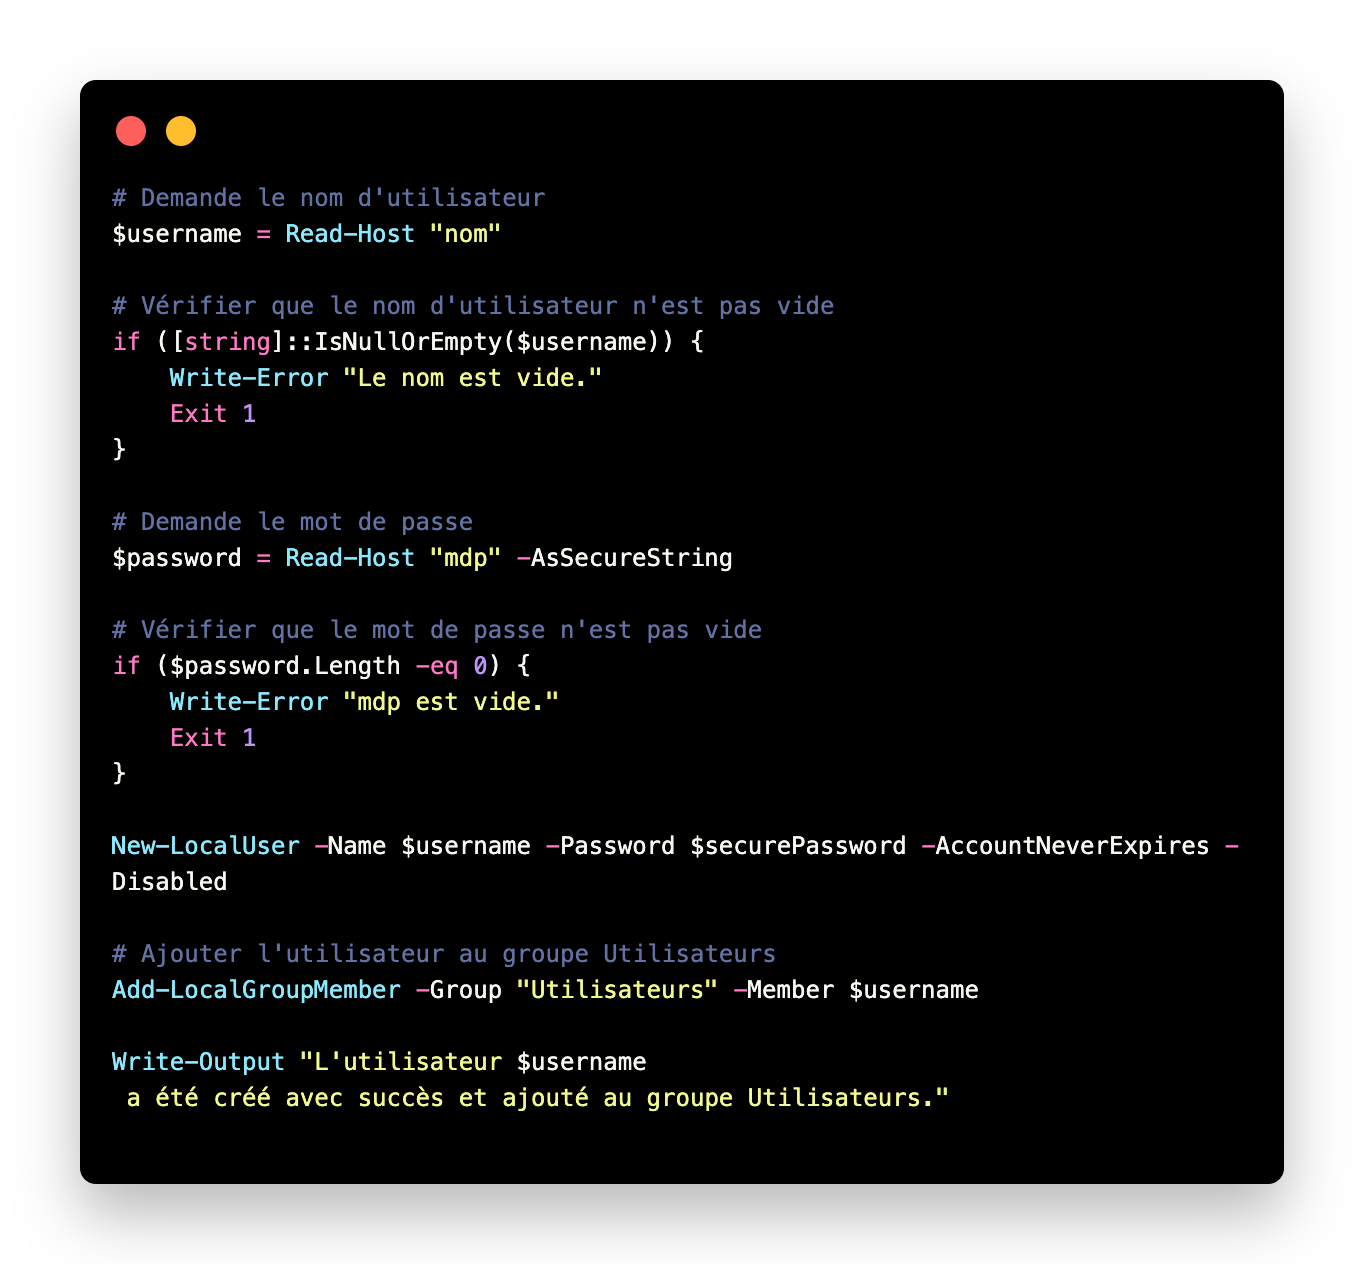
\includegraphics[width=1\textwidth]{img/code1.png}
    \caption{Script création d'utilisateur}
    \label{fig:script1}
\end{figure}

\newpage
\subsection{Exercice 4 - Écrire un script qui affiche le nom d’utilisateur avec la date de sa dernière connexion}
Pour pouvoir afficher la dernière connexion des utilisateurs il suffit de faire 
la commande suivante \textbf{Get-LocalUser | Select-Object Name, LastLogOn}.\\
Le script nous renverra alors un tableau avec les noms d'utilisateurs et leurs 
date et heure de dernière connexion. 

\subsection{Exercice 5}
\subsubsection*{Consigne}

Écrire un script qui se nomme verifie\_doublon.ps1 et qui vérifie si le 
groupe ou l’utilisateur existe. Le programme prendra en paramètre le nom 
d’utilisateur ou de groupe que l’on pourra distinguer avec une option 
(-g pour groupe ou -u pour utilisateur). Voici donc ci-après le script demandé,
avec le bon choix de l'option en fonction -g ou -u... 

\begin{figure}[h]
    \centering
    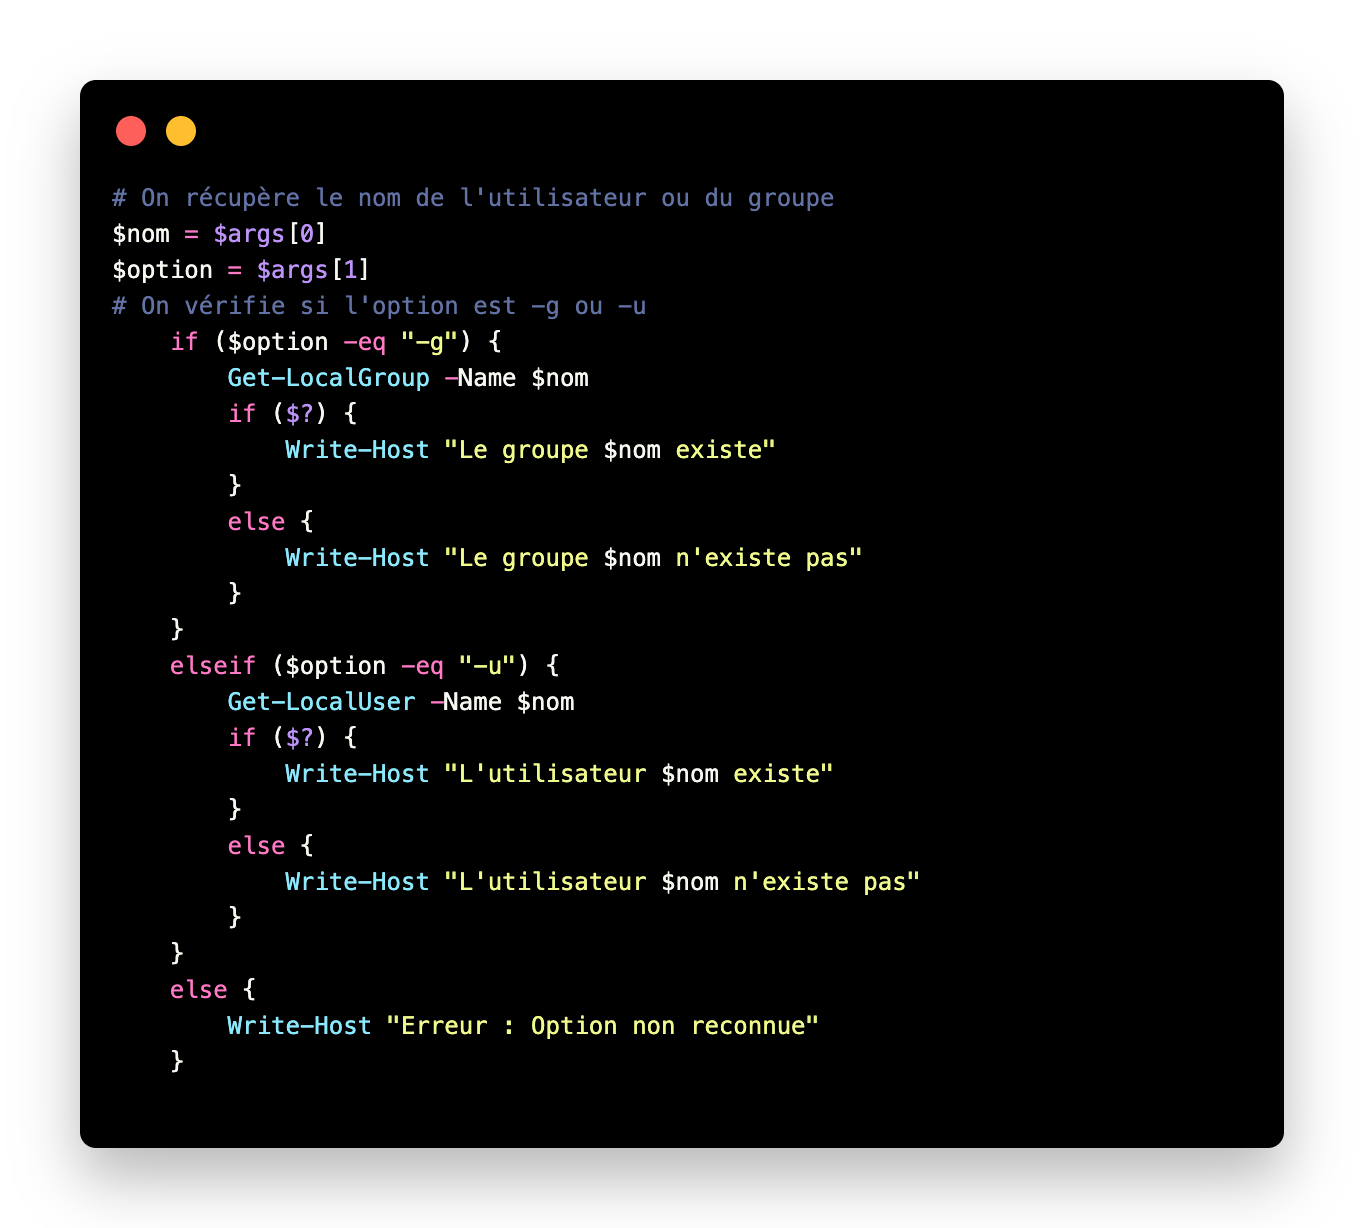
\includegraphics[width=0.8\textwidth]{img/code2.png}
    \caption{verifie\_doublon.ps1}
    \label{fig:script2}
\end{figure}

\newpage
\section{Gestion des logs}
\subsection{Exercice 6 - Quelle option permet d’afficher la liste des logs disponibles ?}
La commande permettant d'afficher les logs disponibles est \textbf{Get-EventLog -List}

\subsection{Exercice 7 - Afficher les sources du log système, sans doublon de préférence}
Pour afficher les sources du log système comme demamdé il suffit de faire la
commande suivante : \textbf{Get-EventLog -LogName System | Select-Object -Property Source -Unique}.
Le script nous renverra alors une liste avec les sources du log système. L'option 
\textbf{-Unique} permet de supprimer les doublons.\\

En rajoutant \textbf{| Measure-Object} à la fin de la commande on peut voir qu'il y a 
24 logs différents.

\subsection{Exercice 8}
\begin{figure}[h]
    \centering
    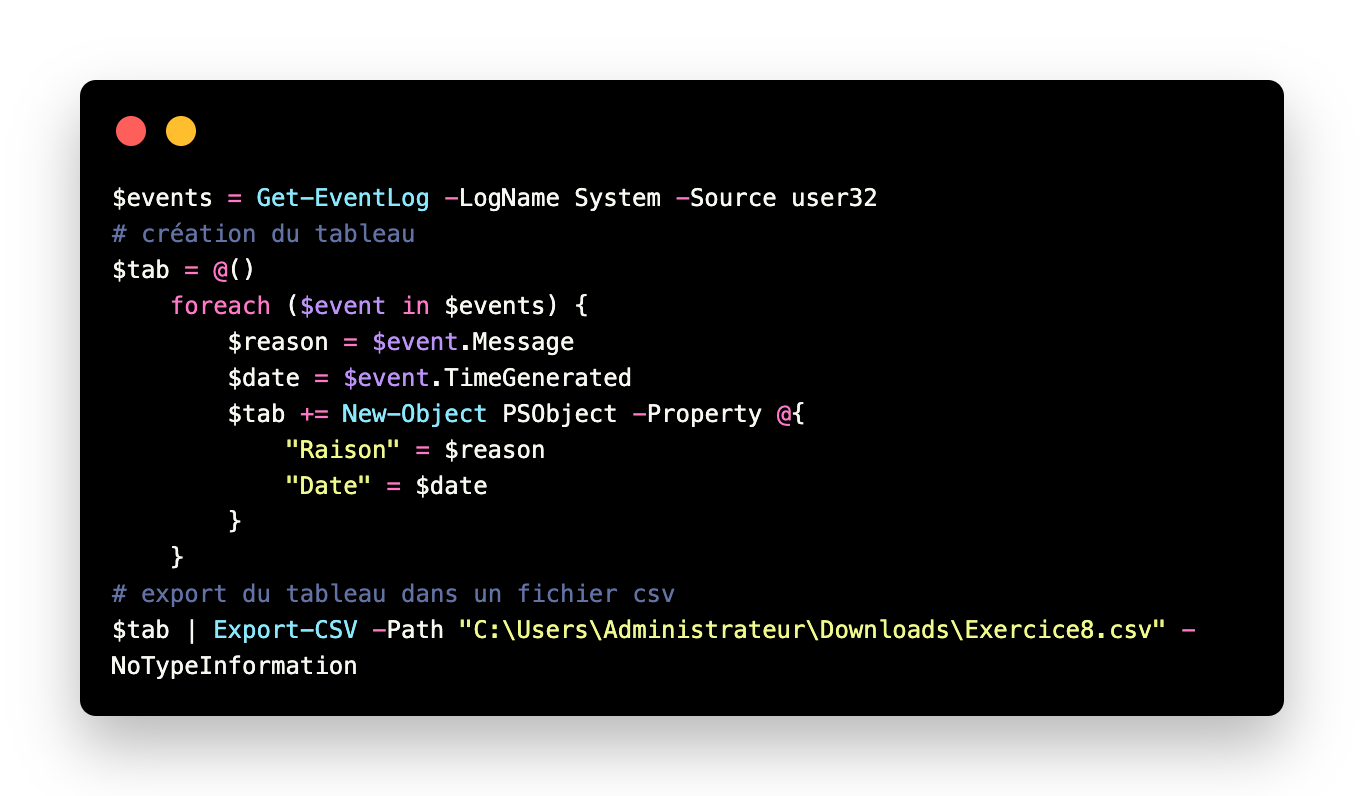
\includegraphics[width=1\textwidth]{img/code3.png}
    \caption{Script CSV}
    \label{fig:script3}
\end{figure}




\end{document}